\newpage
	\textbf{Ejemplo 10}\newline
Supongamos que faltando 10 días para el vencimiento el inversionista del ejemplo anterior decide venderlo y para esta época se están negociando en Bolsa con una tasa del 28\% período 10 días vencido, por lo tanto la tasa de registro debe ser del 28\% período 10 días Vencido. El valor de compra del ejemplo anterior es de 97,204\% COP (faltando 40 días) Suponer el año de 365 días. Calcular:\\
1. El precio de registro en bolsa. \\
2. La retención en la fuente que debe reconocer al vendedor. \\
3. La tasa del vendedor. \\
4. El precio de vendedor. \\
5. Valor de venta.  \\
6. Tasa del comprador. \\
7. Valor del comprador. \newline
\textbf{Solución.
\newline}
\begin{center}
    \renewcommand{\arraystretch}{1.5}% Margenes de las celdas
    %Creación de la cuadricula
    \begin{longtable}[H]{|c|c|c| }
        %Creamos una linea horizontal
        \hline
        %Definimos el color de la primera fila
        \rowcolor[HTML]{FFB183}
        %%%%% INICIO ASIGNACIÓN FECHA FOCAL %%%%%%%
        %%%%%%%%%% INICIO TITULO
        %Lo que se hace aquí es mezclar las 3 columnas en una sola
        \multicolumn{3}{|c|}{\cellcolor[HTML]{FFB183}\textbf{1. Asignación período focal}}   \\ \hline
        %%%%%%%%%% FIN TITULO
        %%%%% INICIO DECLARACIÓN DE VARIABLES %%%%%%%
        \multicolumn{3}{|c|}{$pf = 10 pdv $} \\ \hline
        %Definimos el color de la primera fila
        \rowcolor[HTML]{FFB183}
        %%%%% INICIO DECLARACIÓN DE VARIABLES %%%%%%%
        %%%%%%%%%% INICIO TITULO
        \multicolumn{3}{|c|}{\cellcolor[HTML]{FFB183}\textbf{2. Declaración de variables}}                                                                                   \\ \hline
        %%%%%%%%%% FIN TITULO
        %%%%%%%%%% INICIO DE MATEMÁTICAS
        $F =  100 COP  $ & 
        \multicolumn{2}{c|}{$ a) P_{r} =  ? COP;$\hspace{0.5cm}$ b) i_{v} =  ? \% pdv $} \\
        $ n = 10/365 = 0,027 pdv $ &
        \multicolumn{2}{c|}{$ c) P_{v} = ? COP;$\hspace{0.5cm}$ d) V_{v} =  ? COP $} \\
        $ n = (40-10)/365 pdv $ &
        \multicolumn{2}{c|}{ $ e) i_{c} = ? \% pdv;$\hspace{0.5cm}$ f) P_{c} = ? COP $ } \\
        $ i_{r} = 28\% 10 pdv $     & 
        \multicolumn{2}{c|}{ $ g) V_{c} = ? COP;$\hspace{0.5cm}$ h) R_{F} = ? COP $ } \\
        $ P_{c1} =  97,204 COP $   & 
        \multicolumn{2}{c|}{ $  $ }
        \\ \hline
        %%%%%%%%%% FIN DE MATEMÁTICAS
        %%%%% FIN DECLARACIÓN DE VARIABLES
        
        
        %%%%% INICIO FLUJO DE CAJA
        \rowcolor[HTML]{FFB183}
        \multicolumn{3}{|c|}{\cellcolor[HTML]{FFB183}\textbf{3. Diagrama de flujo de caja}}                                                                                  \\ \hline
        %Mezclamos 3 columnas y pondremos el dibujo
        %%%%%%%%%%%%% INSERCIÓN DE LA IMAGEN
\multicolumn{2}{|c|}{ 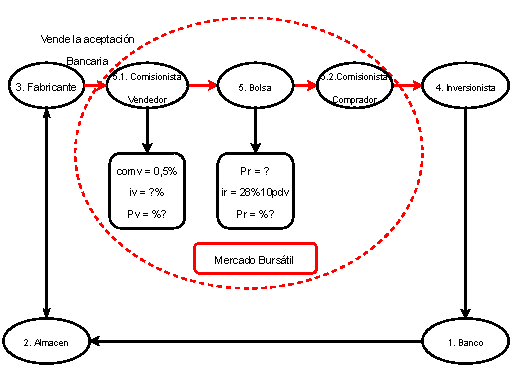
\includegraphics[trim=-90 -5 -90 -5]{3_Capitulo/img/ejemplos/10/capitulo3ejercicio10.pdf} }                                                                                      \\ \hline
        %%%%%%%%%%%%% FIN INSERCIÓN DE IMAGEN
        %%%%%FIN FLUJO DE CAJA
        
        
        
        %%%%% INICIO DECLARACIÓN FORMULAS
        %%%%%%%%%%% INICIO TITULO
        \rowcolor[HTML]{FFB183}
        \multicolumn{3}{|c|}{\cellcolor[HTML]{FFB183}\textbf{4. Declaración de fórmulas}}                                                                                    \\ \hline
        %%%%%%%%%%% FIN TITULO
        %%%%%%%%%%% INICIO MATEMÁTICAS
    
         \multicolumn{3}{|c|}{$P=F(1+i)^{-n}$\hspace{35pt}\textit{Valor presente}
         \hspace{0.3cm}}\\
         \multicolumn{3}{|c|}{$R_{F} = (F - P)*0,7$\hspace{35pt}\textit{Retención en la fuente}
         \hspace{0.3cm}}\\
         \multicolumn{3}{|c|}{$V_{V} = P_{V} * V_{total}$\hspace{35pt}\textit{}
         \hspace{0.3cm}}\\
         \multicolumn{3}{|c|}{$V_{C} = P_{C} * V_{total}$\hspace{35pt}\textit{}
         \hspace{0.3cm}}\\
        
         
         \hline
        %%%%%%%%%% FIN MATEMÁTICAS
        %%%%%% INICIO DESARROLLO MATEMÁTICO
        \rowcolor[HTML]{FFB183}
        %%%%%%%%%%INICIO TITULO
        \multicolumn{3}{|c|}{\cellcolor[HTML]{FFB183}\textbf{5. Desarrollo matemático}}                                                                                      \\ \hline
        %%%%%%%%%% FIN TITULO
        %%%%%%%%%% INICIO MATEMÁTICAS
         \multicolumn{3}{|c|}{$ a) P_{r} = 100 COP * (1 + 0,28)^{-10/365} = 99,3260\% COP$
         \hspace{0.3cm}}\\
         \multicolumn{3}{|c|}{$ b) 97,204 COP = 99.3260 (1+i)^{-30/365} => i_{v} = 6,4\% pdv$
         \hspace{0.3cm}}\\
         \multicolumn{3}{|c|}{$ d) V_{v} = 0,972 COP * 5{.}000{.}000 COP = 4{.}860{.}000 COP $
         \hspace{0.3cm}}\\
         \multicolumn{3}{|c|}{$ e) 99,3260 \% = 100 COP (1+ i)^{-10/365} => i = 9,84\%$
         \hspace{0.3cm}}\\
         \multicolumn{3}{|c|}{$ f) P_{c} = 100 COP (1 + 0,0984)^{-10/365} = 90,16\% COP $
         \hspace{0.3cm}}\\
         \multicolumn{3}{|c|}{$ g) V_{c} = 0,9016 * 5{.}000{.}000 COP = 4{.}508{.}000 COP $
         \hspace{0.3cm}}\\
         \multicolumn{3}{|c|}{$ h) R_{F} = 0,07(5{.}000{.}000 - 97,204) $
         \hspace{0.3cm}}\\
         
        %%%%%%%%%% FIN MATEMÁTICAS
        %%%%%% FIN DESARROLLO MATEMÁTICO
        
        \rowcolor[HTML]{FFB183}
        \multicolumn{3}{|c|}{\cellcolor[HTML]{FFB183}\textbf{6. Respuesta}} \\ \hline    
        
        \multicolumn{3}{|c|}{$P_{r} = 4{.}964{.}190 COP $} \\ \hline
    \end{longtable}
    %Se crean dos lineas en blanco para que no quede el siguiente texto tan pegado
\end{center}